%! TEX root = ../main.tex

\chapter{Monte Carlo simulations and probability density functions}%
\label{apdx:magepdfs}

\blocktitle{MaGe}
Background components that were identified in the energy spectra or in
radio-purity screening measurements (see \cref{apdx:assay}) are
simulated using the \mage\ software~\cite{Boswell2011} based on
\geant~\cite{Agostinelli2002, Allison2006, Allison2016}.  The \gerda\
\phasetwo\ detectors, their arrangement in seven strings as well as the
LAr instrumentation are implemented into \mage. A graphic rendering of
the relevant implemented hardware components is presented
in~\cref{fig:setup:magevolumes}.
\newpar
Simulations of radioactive decays and full tracking of the decay
products are performed in all the hardware components close enough to
the detector. Relevant event data like energy depositions in sensitive
detectors (germanium, LAr, SiPMs and PMTs), hit location in germanium
and LAr is written on disk. Propagation of optical photons
(e.g.~resulting from the LAr scintillation) is disabled by default to
save computing time. It is only enables during special simulations of
the LAr veto capabilities.  The built-in \geant\ generators and
databases are used to simulate all radioactive decays except for
double-beta decay in germanium, for which more details about the decay
dynamics (e.g.~angular correlations between the emitted electrons) are
needed. The primary spectrum of the two electrons is indeed sampled in a
separate step according to the distribution given in
reference~\cite{Tretyak1995} implemented in
\decayzero~\cite{Ponkratenko2000}.
\newpar
The \kvz\ decays (except for surface contaminations) are simulated
homogeneously distributed in the relevant LAr volume. The following LAr
volumes are chosen for the background model: the first is a cylinder
centered on the detector array ($h=250$~cm, $r=100$~cm, simply referred
to as ``homogeneous'' or shortened to ``hom.''~in the following)
subsequently divided into the volume enclosed by the mini-shrouds and
the remaining one (outside the mini-shrouds); the second is a cylinder
($h=100$~cm, $r=25$~cm) positioned just above the array and the
remaining seven are smaller cylinders ($h=20$~cm, $r=5$~cm), each one
positioned just above each of the seven detector strings.

\blocktitle{pdfs}
The output of \mage\ simulations is further processed to compute the
probability density functions (pdfs) used to model the \gerda\ data in
the statistical analysis. This procedure includes folding in run-time
dependent information, i.e.~the detector status in each physics run, the
finite energy resolution and threshold of each detector. The detector
dead-layer model is also applied in this post-processing step, by
re-weighting energy positions according to their distance from the
nearest surface. All pdfs presented in the following are computed using
the run-time parameters of the data sets they refer to. A selection of
the pdfs projected in energy space and normalized to the number of
simulated events, is displayed in \cref{fig:bkg:raw:ph2:pdfs:gmodel}.

For the potassium tracking analysis pdfs binned in detector space are
used to model the data. The rotationally symmetric single-detector pdfs
for the \kvn\ and \kvz\ energy windows are shown in
\cref{fig:bkg:raw:ph2:pdfs:kmodel:K42} and
\cref{fig:bkg:raw:ph2:pdfs:kmodel:K40}.  For two-detector events the
following representation style is used:
projections of the two-dimensional histograms on their axis are summed,
such that each two-detector event enters the final histogram twice, in
the two bins associated to the respective detectors. They can be found
in \cref{fig:bkg:raw:ph2:pdfs:kmodel:K40} together with the single-detector
pdfs of the rotationally asymmetric components. 

Common features can be noticed across the multitude of histogram shapes.
The event rate in single-detector data is generally higher in coaxial
detectors, due to their larger mass compared to BEGe detectors ---
maximal correlation between event rate and detector-by-detector exposure
can be found in the \nnbb\ pdf in~\cref{fig:bkg:raw:ph2:pdfs:kmodel:K42}. This
feature is generally lost in the two-detector data: the coaxial
detectors larger volume allows to stop more efficiently
$\gamma$-particles that would otherwise escape and eventually deposit
energy in a second detector. Other similarities between different pdfs
can be attributed to detectors live-times, like in the case of
\texttt{GD91C}, which was inactive for a large fraction of the
\phasetwo\ exposure and thus generally registers a low number of counts.
The effects of asymmetrically distributed background contaminations are
easily recognizable in the shape of the pdfs.  Impurities located above
the detector array are mostly seen by the upper most detectors in each
string as can be seen for \kvn\ in the front-end electronics
in~\cref{fig:bkg:raw:ph2:pdfs:kmodel:K40:M1} and
in~\cref{fig:bkg:raw:ph2:pdfs:kmodel:K40:M2} and for \kvz\ above each
mini-shroud (see~\cref{fig:bkg:raw:ph2:pdfs:kmodel:K42sep:M1} and
\cref{fig:bkg:raw:ph2:pdfs:kmodel:K40sep:M2}). Rotationally asymmetric
components are mostly evident in a single string, see for example \kvn\
in single mini-shrouds in \cref{fig:bkg:raw:ph2:pdfs:kmodel:K40sep:M1} and
\cref{fig:bkg:raw:ph2:pdfs:kmodel:K40sep:M2}.

\begin{figure}
  \centering
  \subfloat[%
    \kvn\ in different setup locations and \nnbb\ in Ge,
    \Mokvn\ data set.\label{fig:bkg:raw:ph2:pdfs:kmodel:K40:M1}%
  ]{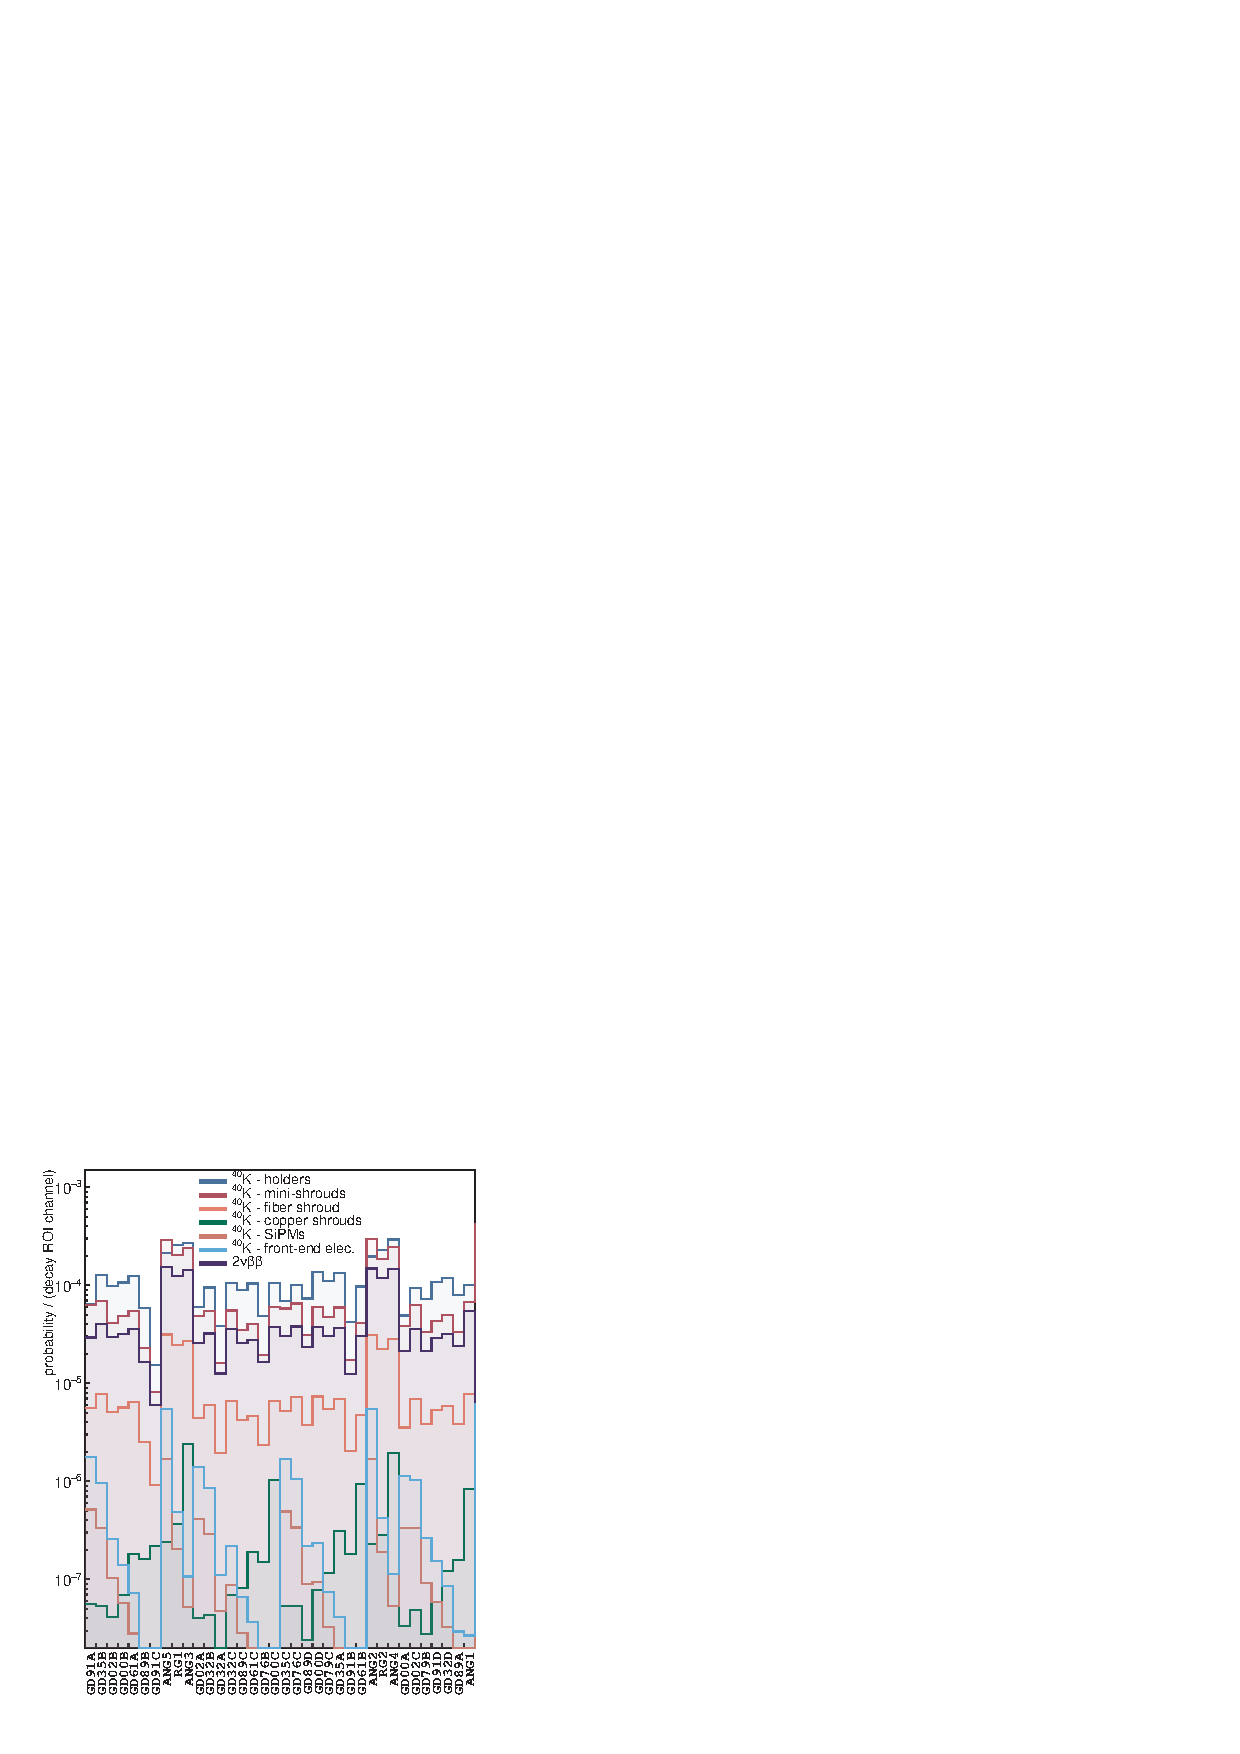
\includegraphics[width=0.48\textwidth]{plots/bkg/raw/ph2/pdfs/kmodel-pdfs-K40.pdf}}
  \hfill
  \subfloat[%
    \kvn\ located close to each single mini-shroud, \Mokvn\
    data set.\label{fig:bkg:raw:ph2:pdfs:kmodel:K40sep:M1}%
  ]{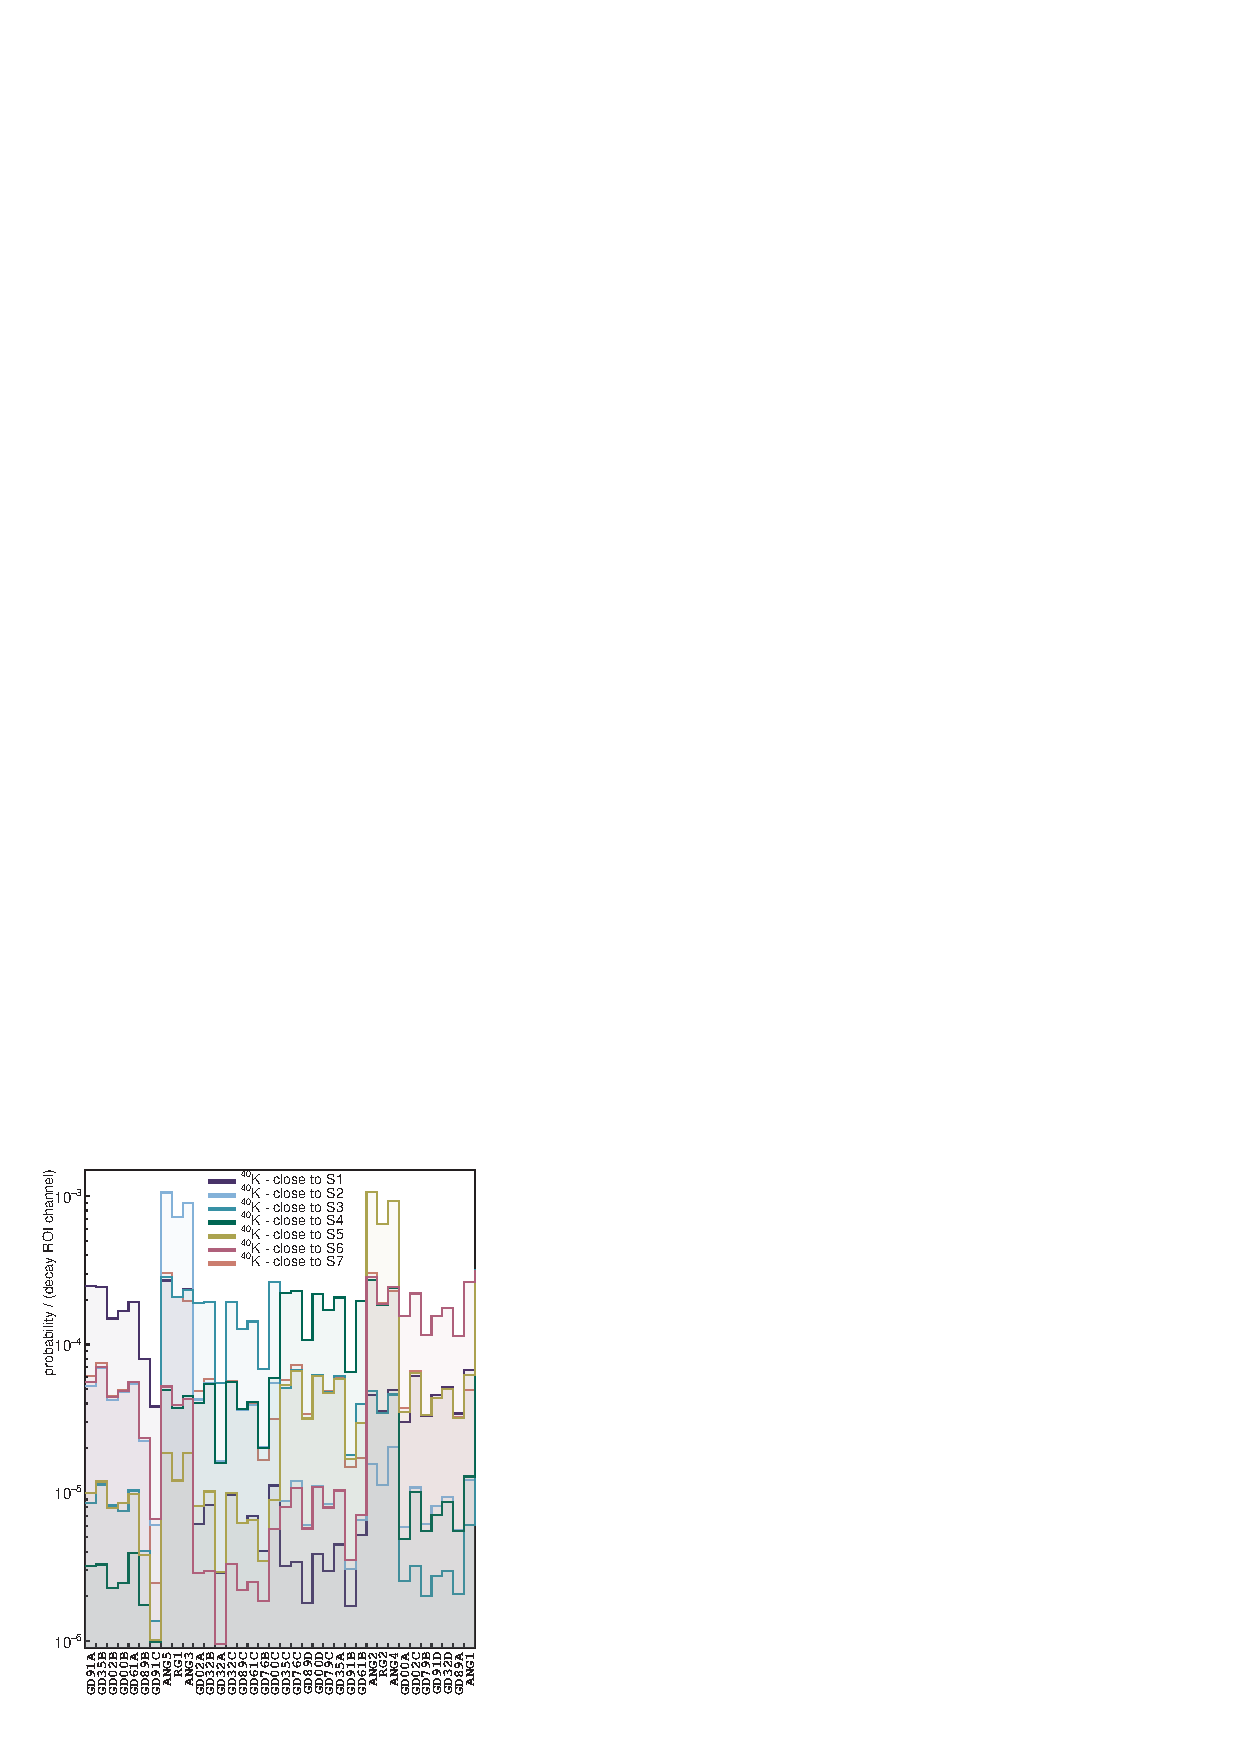
\includegraphics[width=0.48\textwidth]{plots/bkg/raw/ph2/pdfs/kmodel-pdfs-K40-sep.pdf}}

  \subfloat[%
    \kvn\ in different setup locations, \Mtkvn\
    data set.\label{fig:bkg:raw:ph2:pdfs:kmodel:K40:M2}%
  ]{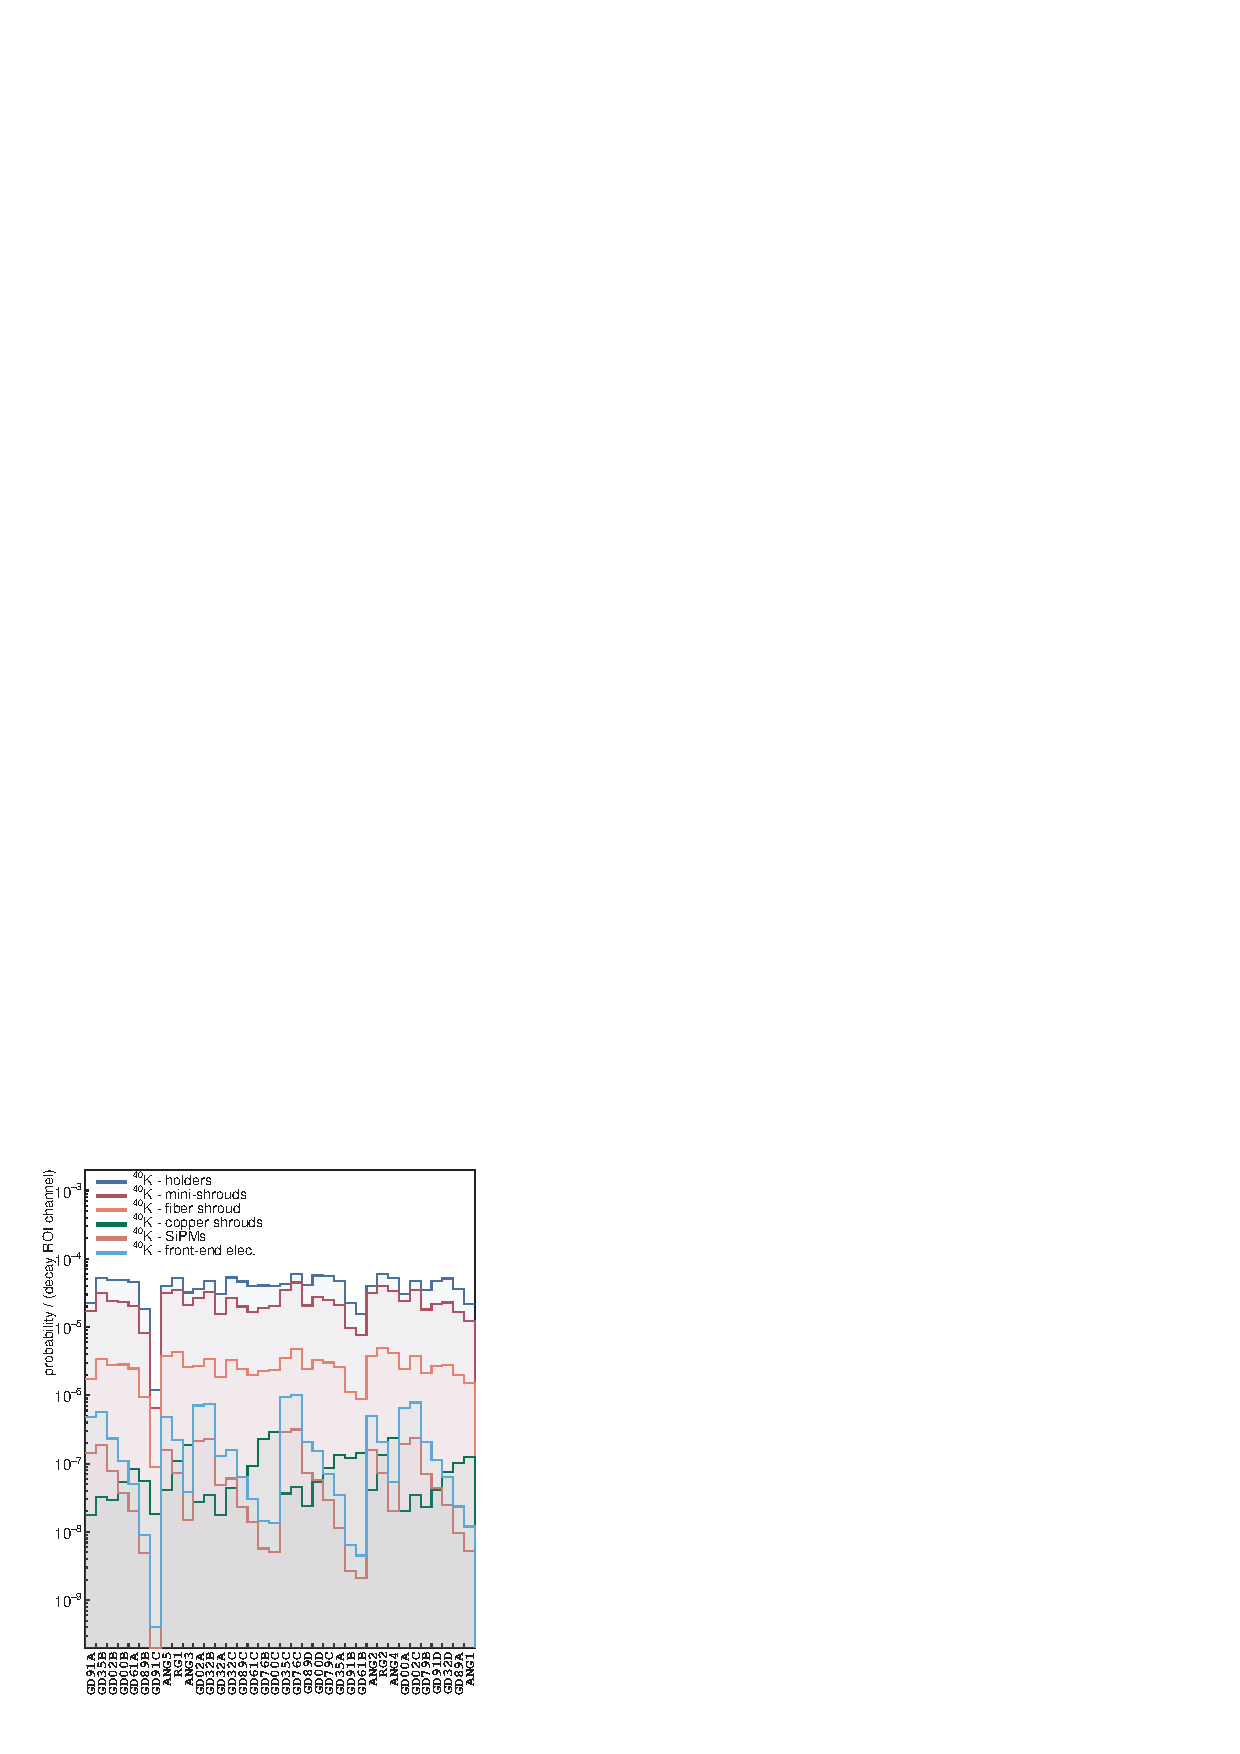
\includegraphics[width=0.48\textwidth]{plots/bkg/raw/ph2/pdfs/kmodel-pdfs-K40-M2.pdf}}
  \hfill
  \subfloat[%
    \kvn\ located close to each single mini-shroud, \Mtkvn\
    data set.\label{fig:bkg:raw:ph2:pdfs:kmodel:K40sep:M2}%
  ]{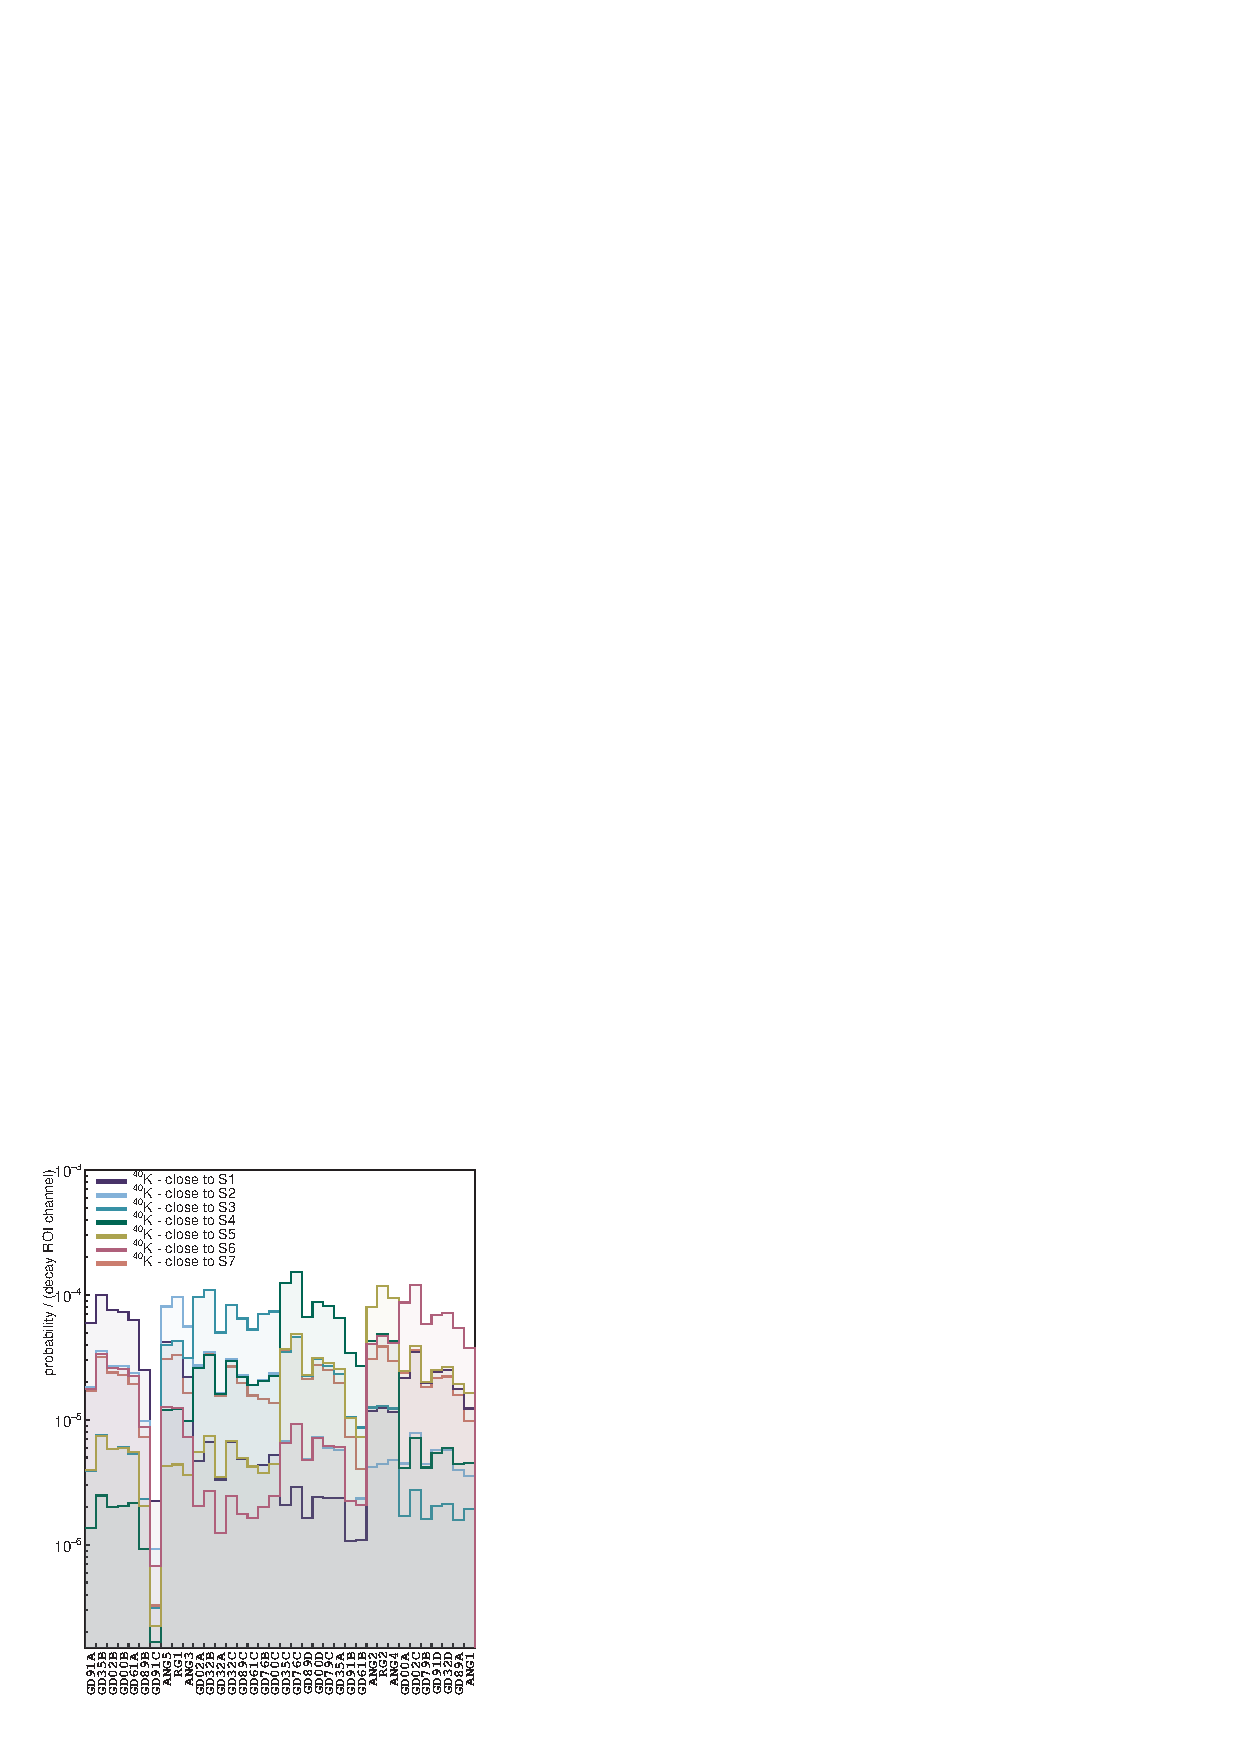
\includegraphics[width=0.48\textwidth]{plots/bkg/raw/ph2/pdfs/kmodel-pdfs-K40-sep-M2.pdf}}

  \caption{%
    pdfs binned in detector space for the \kvn\ tracking analysis. 
    All pdfs are normalized to the number of simulated primary decays.
  }\label{fig:bkg:raw:ph2:pdfs:kmodel:K40}
\end{figure}

\begin{figure}
  \subfloat[%
    \kvz\ in different setup locations and \nnbb\ in Ge,
    \Mokvz\ data set.\label{fig:bkg:raw:ph2:pdfs:kmodel:K42:M1}%
  ]{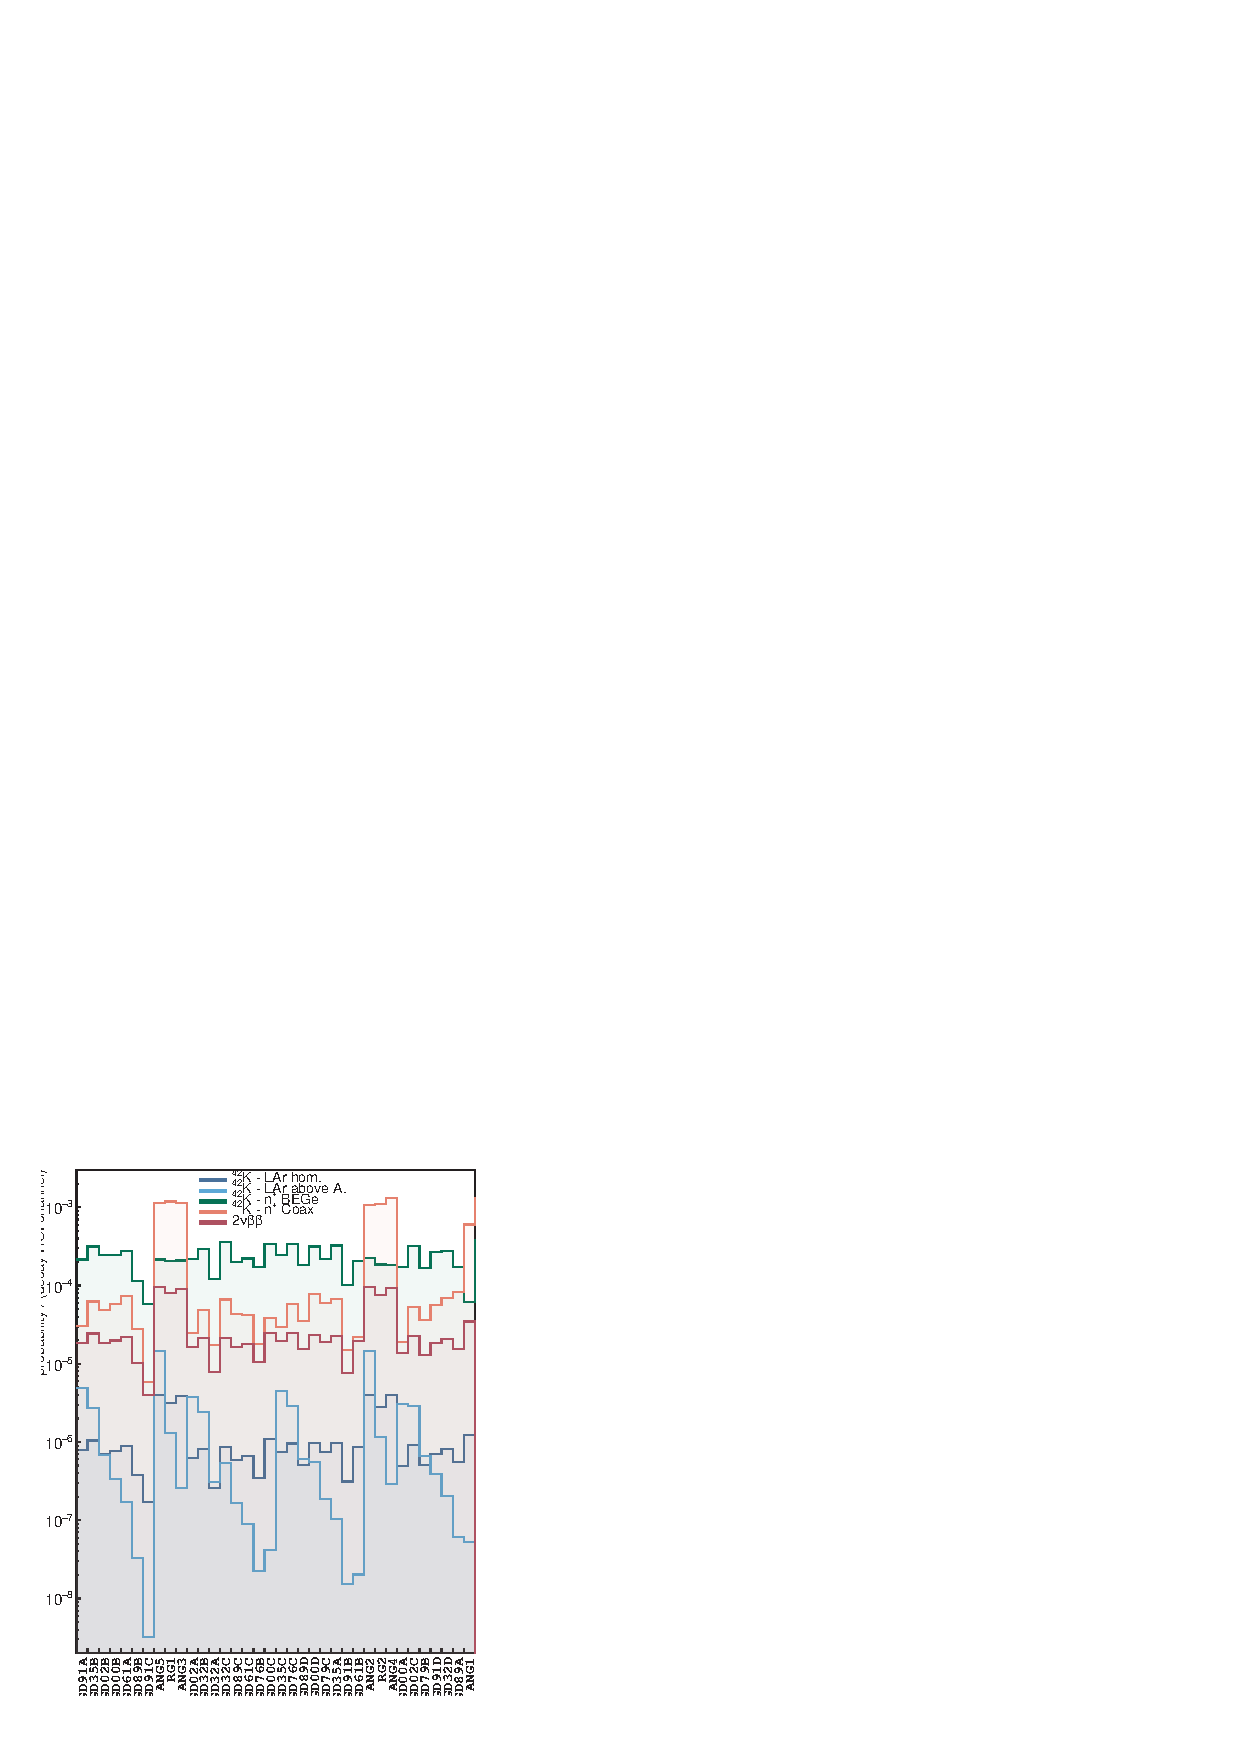
\includegraphics[width=0.48\textwidth]{plots/bkg/raw/ph2/pdfs/kmodel-pdfs-K42.pdf}}
  \hfill
  \subfloat[%
    \kvz\ in LAr above each single mini-shroud, \Mokvz\
    data set.\label{fig:bkg:raw:ph2:pdfs:kmodel:K42sep:M1}%
  ]{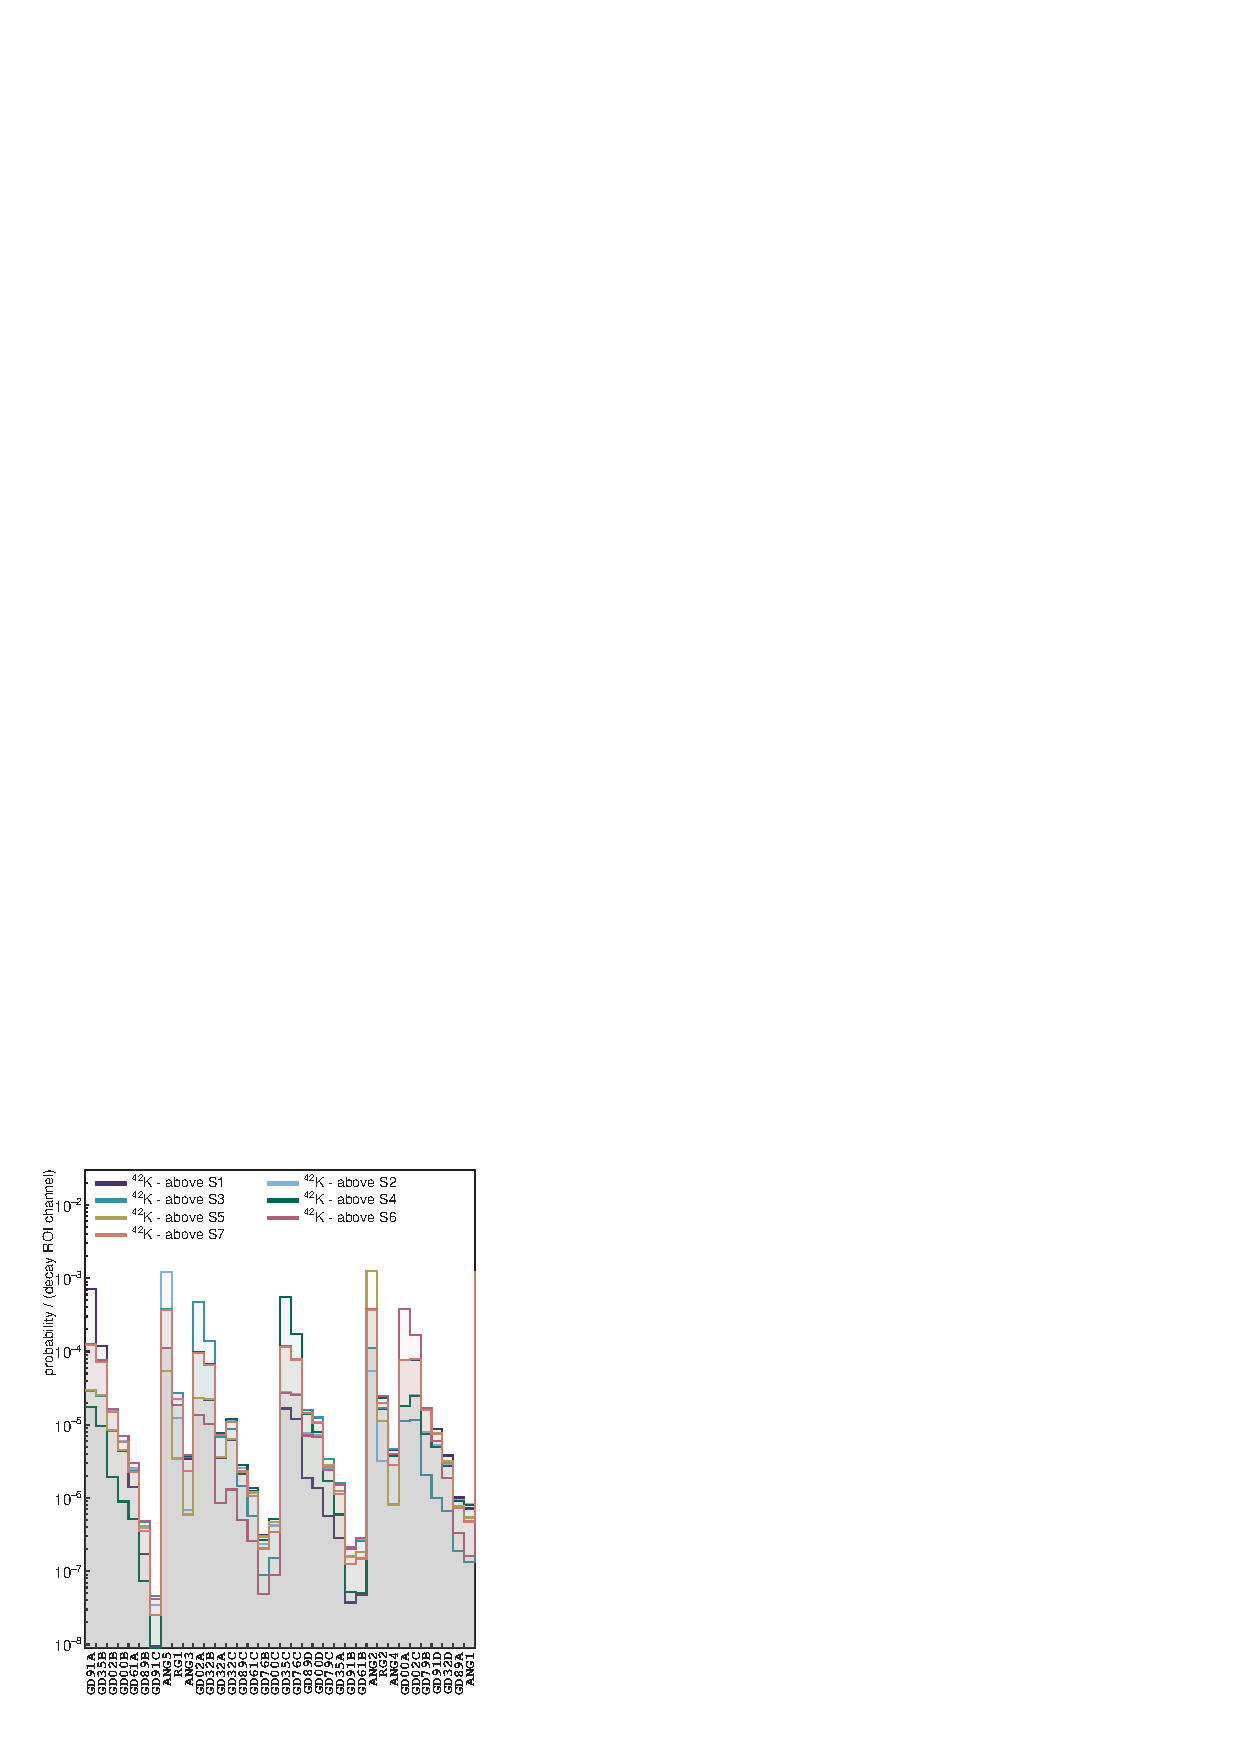
\includegraphics[width=0.48\textwidth]{plots/bkg/raw/ph2/pdfs/kmodel-pdfs-K42-sep.pdf}}

  \subfloat[%
    \kvz\ in different setup locations, \Mtkvz\
    data set.\label{fig:bkg:raw:ph2:pdfs:kmodel:K42:M2}%
  ]{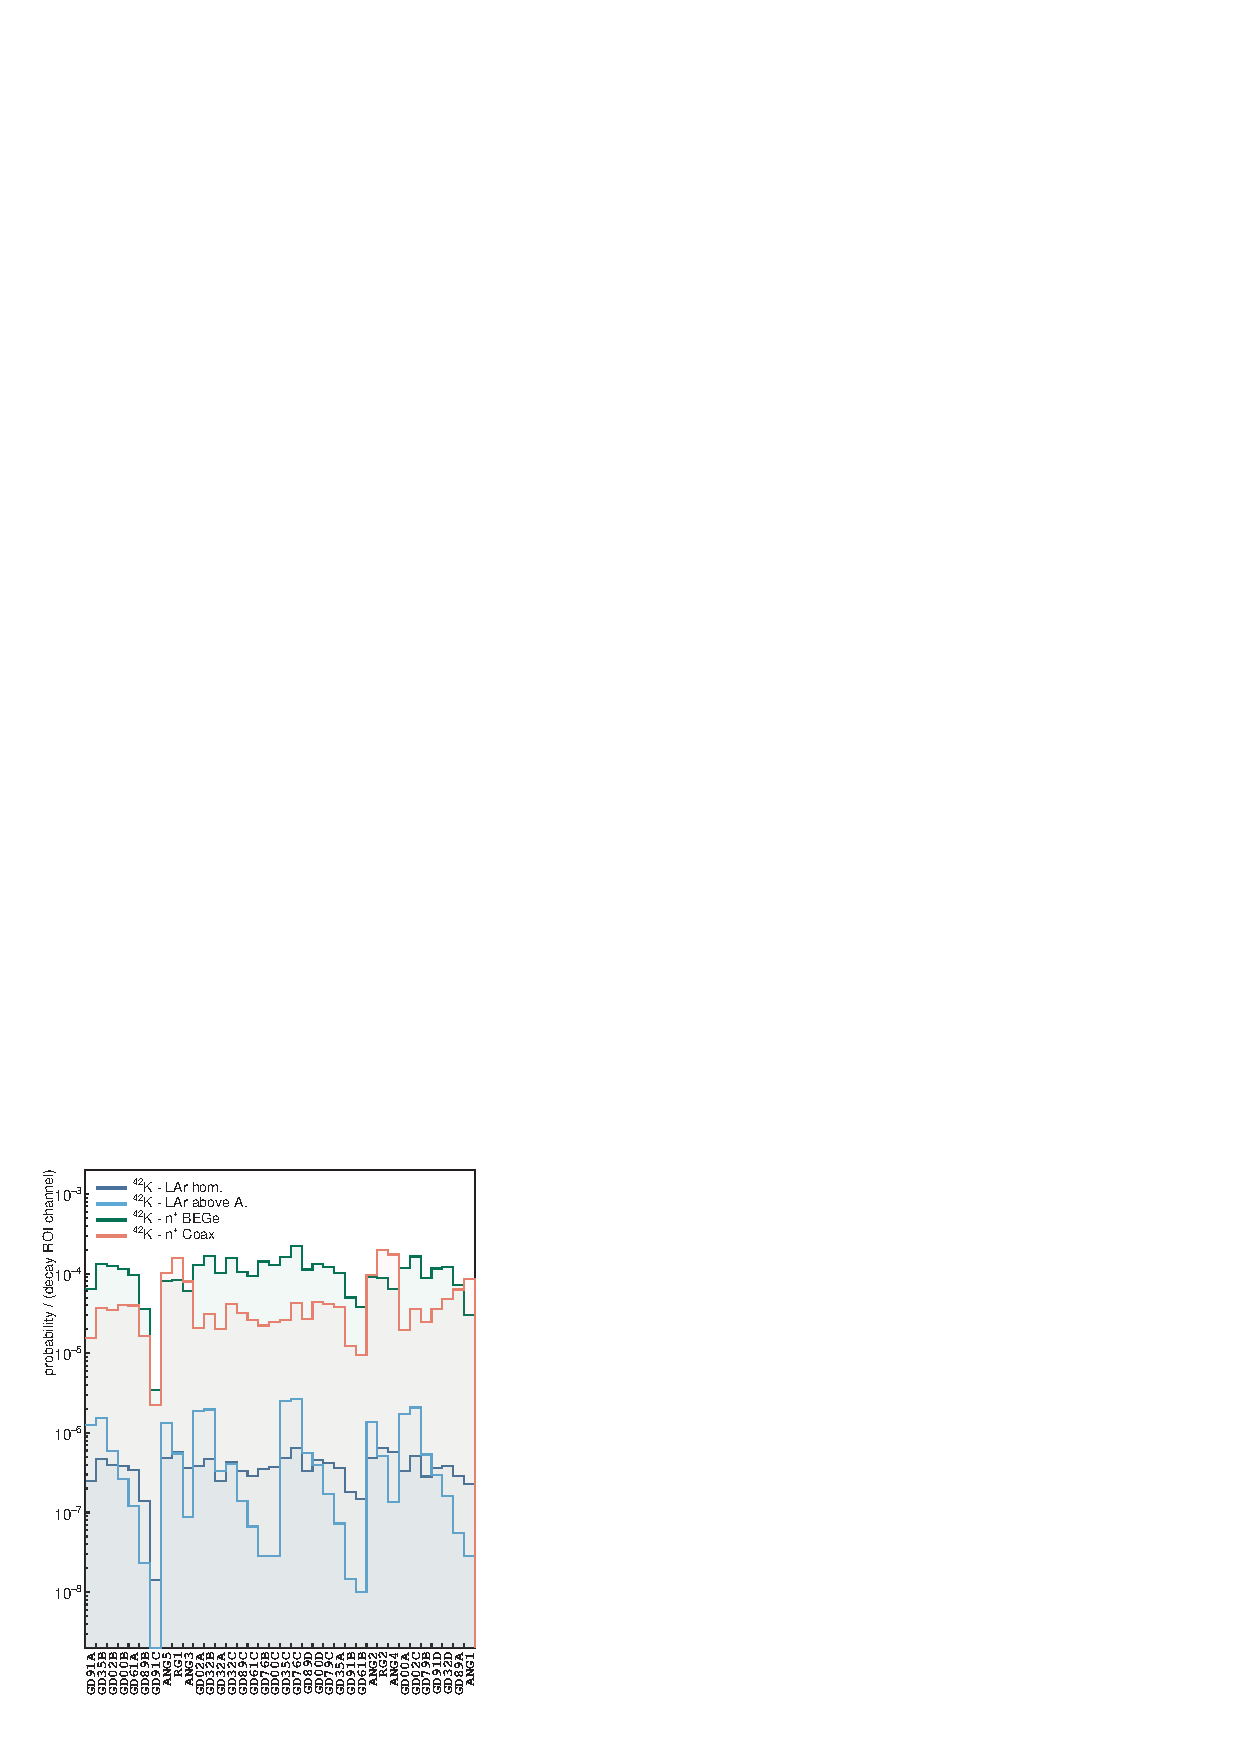
\includegraphics[width=0.48\textwidth]{plots/bkg/raw/ph2/pdfs/kmodel-pdfs-K42-M2.pdf}}
  \hfill
  \subfloat[%
    \kvz\ in different setup locations, \Mtkvz\
    data set.\label{fig:bkg:raw:ph2:pdfs:kmodel:K42sep:M2}%
  ]{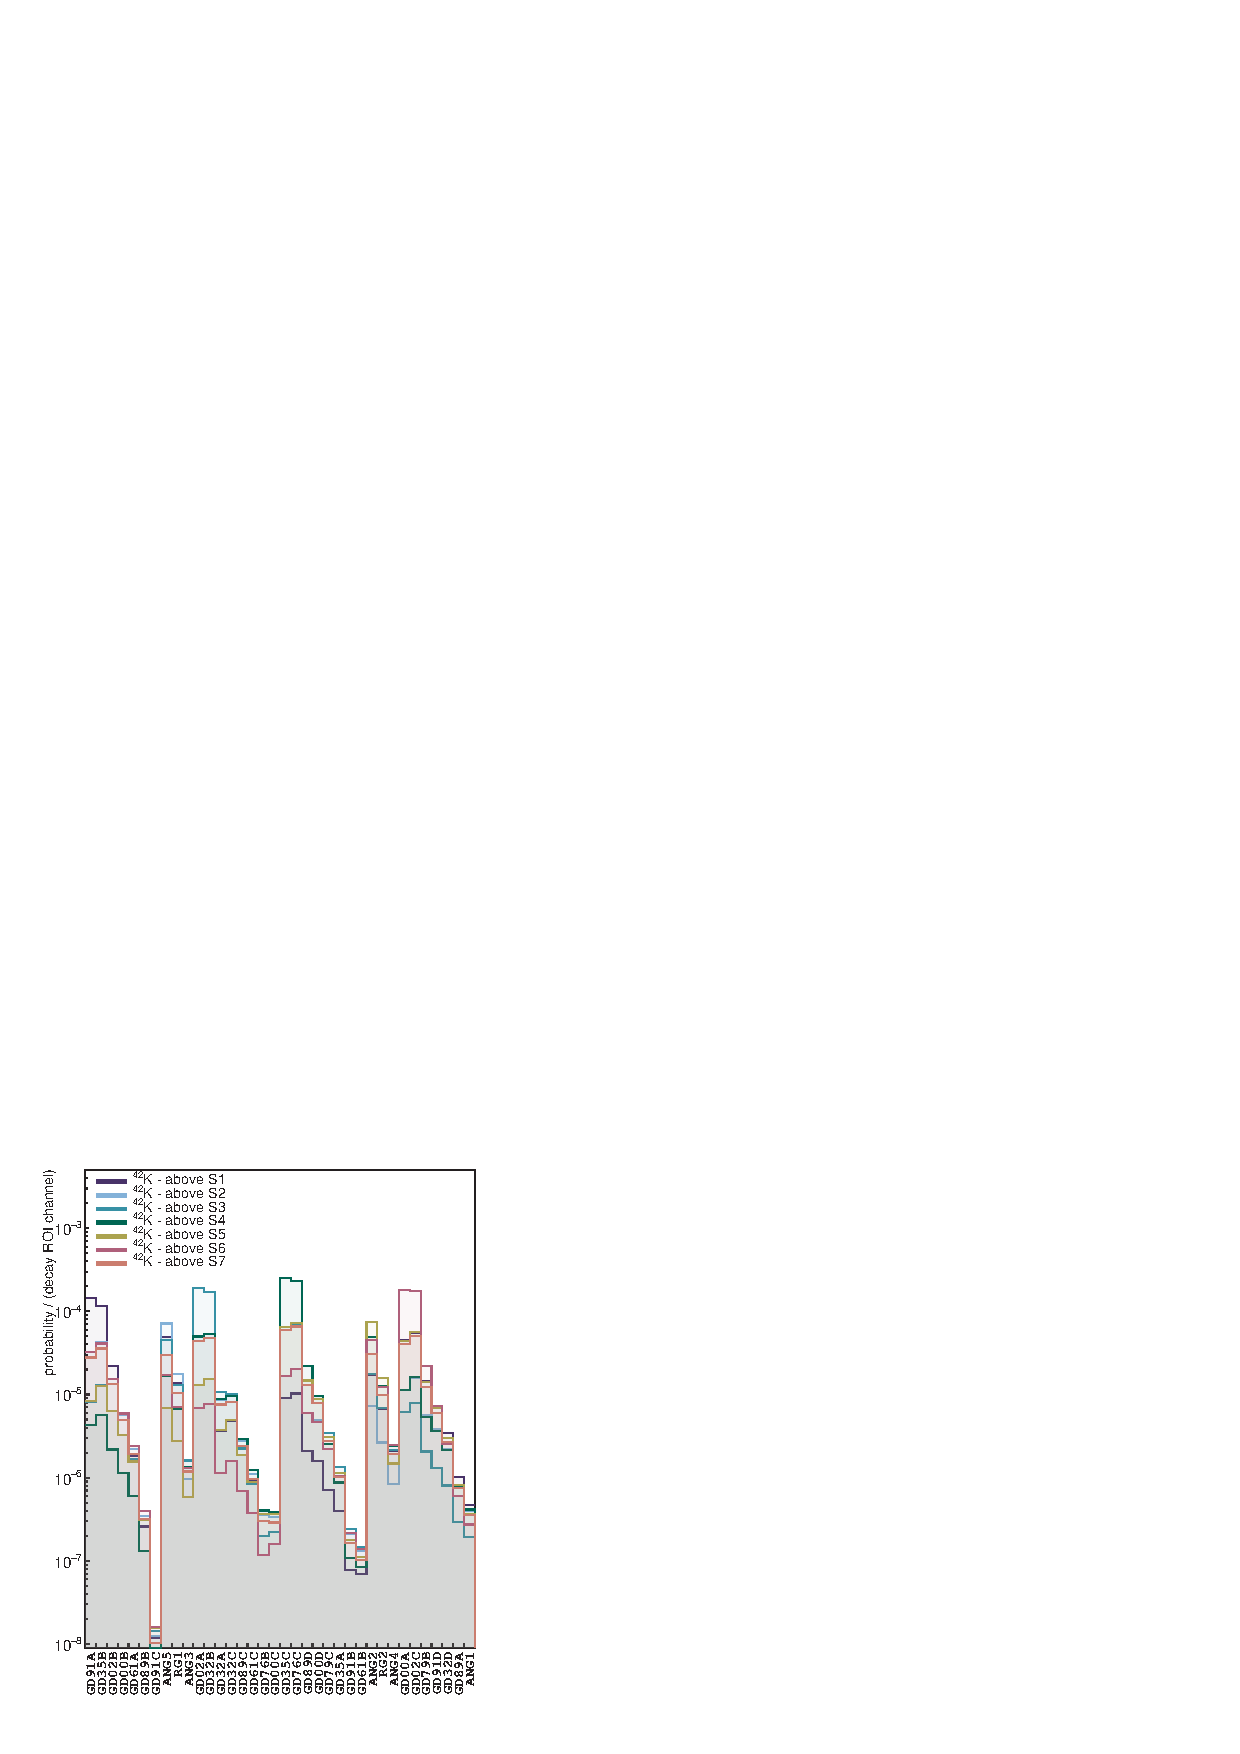
\includegraphics[width=0.48\textwidth]{plots/bkg/raw/ph2/pdfs/kmodel-pdfs-K42-sep-M2.pdf}}

  \caption{%
    pdfs binned in detector space for the \kvz\ tracking analysis. 
    All pdfs are normalized to the number of simulated primary decays.
  }\label{fig:bkg:raw:ph2:pdfs:kmodel:K42}
\end{figure}

All \a\ decays in the \Ra\ to \Pbl\ sub-chain and from \Po\ are
simulated on the \pplus\ detector surface separately and for different
thicknesses of the \pplus\ electrode. The \Ra\ chain is simulated
together under the assumption that in each \a\ decay half of the
contamination is lost due to the recoil of the nucleus into the LAr. The
resulting pdfs are displayed in~\cref{fig:bkg:raw:ph2:pdfs:amodel:Po}
and \cref{fig:bkg:raw:ph2:pdfs:amodel:Ra}. The spectra exhibit a peak
like structure with a pronounced low-energy tail.  The maximum is
shifted with respect to the full emission energy due to the thickness of
the \pplus\ contact.  The low-energy tail is characteristic for \a\
decays; the \a\ particle is susceptible to the change in the contact
thickness when penetrating the detector surface under an incident angle
and loses part of its energy before reaching the active detector volume.

% vim: tw=72 tabstop=2 expandtab shiftwidth=2
